
\chapter{Configuration, Settings and Preferences}%
\label{cha:configuration_settings_preferences}

\begin{figure}[htpb]
    \centering 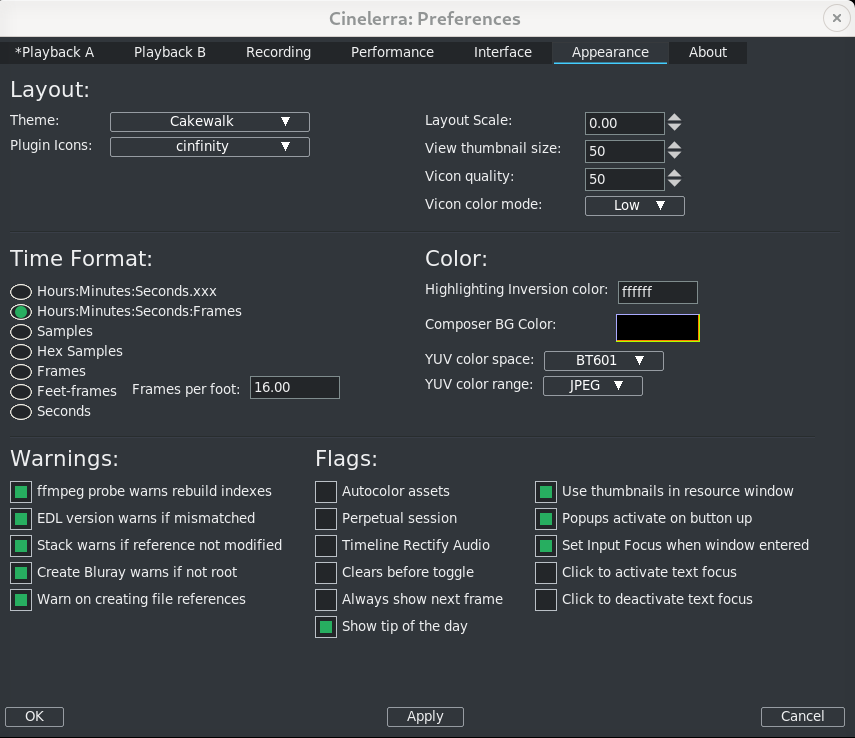
\includegraphics[width=0.9\linewidth]{images/settings.png}
    \caption{Settings of default Preferences with the Appearance tab selected}
    \label{fig:settings}
\end{figure}

The user's default settings, preferences, and other helpful files are retained across sessions in a hidden file, called .bcast5, in the user’s \texttt{\$HOME} directory. Initially when Cinelerra is launched there is an empty project and there are program default settings, and from then on the \texttt{.bcast5} directory will contain the settings that were set when quitting.  If you need to revert to the default settings, delete the \texttt{.bcast5} directory contents and restart Cinelerra.  Or you may want to rename it temporarily if you think you might want it back later.
Although the location defaults to \texttt{\$HOME/.bcast5}, you can use the \texttt{CIN\_CONFIG} variable to override this location.  For example:  \texttt{export CIN\_CONFIG=/tmp/.bcast5}  will use a temporary setup for testing purposes.  It is also useful for multiple users sharing the same home directory who would like to have different configuration/preferences settings data.  And if you are experiencing inexplicable errors or crashes in Cinelerra, they may be due to a problem with \texttt{.bcast5} in which case taking it out of the picture  can at least eliminate this as the cause.

Several ways exist to change Cinelerra’s operational characteristics.  A lot of variations can be made to  settings and preferences by using the \textit{Settings} pulldown from the main window and choosing \textit{Preferences}.

\section{Playback A / Playback B}%
\label{sec:playback_a_b}

\subsection{Audio Out section}%
\label{sub:audio_out_section}

The audio drivers are used for both recording and playback. The Audio Out settings affect the outcome when you play sound on the timeline.

\begin{description}
    \item[Playback buffer samples] for playing audio, small fragments of sound are read from disk and processed sequentially. A larger value here causes more latency when you change mixing parameters but yields more reliable playback.  Some sound drivers do not allow changing of the fragment, so latency is unchanged no matter what the value. Since different stages of the rendering pipeline can change the rate of the incoming data, it would be difficult to disconnect the size of the console fragments from the size of the fragments read from disk.
    \item[Audio offset (sec)] the ability to tell the exact playback position on Linux sound drivers is poor.  The audio offset allows users to adjust the position returned by the sound driver in order to reflect reality. The audio offset does not affect the audio playback or rendering at all. It merely changes the synchronization of video playback. The easiest way to set the audio offset is to create a timeline with one video track and one audio track. Expand the audio track and center the audio pan. The frame rate should be larger than $24 fps$ and the sampling rate should be greater than $32000$. The frame size should be small enough for your computer to render it at the full framerate. Highlight a region of the timeline starting at 10 seconds and ending at 20 seconds. Drop a gradient effect on the video track and configure it to be clearly visible. Drop a synthesizer effect on the audio and configure it to be clearly audible. Play the timeline from 0 and watch to see if the gradient effect starts exactly when the audio starts. If it does not, expand the audio track and adjust the nudge. If the audio starts ahead of the video, decrease the nudge value. If the audio starts after the video, increase the nudge value. Once the tracks play back synchronized, copy the nudge value to the audio offset value in preferences. Note: if you change sound drivers or Disable hardware synchronization, you will need to change the audio offset because different sound drivers are unequally inaccurate.
    \item[View follows playback] this causes the timeline window to scroll when the playback cursor moves. This can slow down the X Server or cause the timeline window to lock up for long periods of time while drawing the assets.
    \item[Disable hardware synchronization] most sound cards and sound drivers do not give reliable information on the number of samples the card has played. You need this information for synchronization when playing back video. This option causes the sound driver to be ignored and a software timer to be used for synchronization.
    \item[Audio playback in realtime priority (root only)] for really old computers, this setting allows uninterrupted playback during periods of heavy load. It forces the audio playback to the highest priority in the kernel. Today, it is most useful for achieving very low latency between console tweaks and sound card output. You must be root to get real-time priority. Only experts might want to use this because it interferes with ordinary time-share scheduling and can lock up the system.  When this is enabled, audio gets the first shot and burns audio until audio lets go. To explain, there are 2 kinds of scheduling, \textit{time-sharing} which is the default, and \textit{real time} where the scheduled task must explicitly request scheduling to allow other tasks to execute.  Time-share interrupts when you use up your allocated time slice.  Realtime priority audio will execute audio decode until it finishes, which may slow down other types of processing like video decoding.  Most decoders use a policy that video may be downsampled to accommodate scheduling, but will never skip audio because it creates a much more obvious defect.  This feature helps to make sure audio gets priority over video during decode. Be sure to check apply in order for this feature to take effect.
    \item[Map 5.1$\rightarrow$2] playback 5.1 $\rightarrow$ 2 driver downmix maps 6 tracks to 2 channels when checked, that is mixes $5.1$ down to stereo on the output device side.  This is different from the patchbay and menubar functions which reset the pan/mix levels of the input channels.  In this way, you can render $5.1$ media, and use stereo speakers to listen in the same session setup.  This downmix only occurs if the playback is $5.1$ (6 channels) and the device config is stereo (2 channels).
    \item[Gain] set audio gain to a different value than the default of $1.0$ This feature, device level gain, corrects for hardware conditions which some devices may need to be useful.  For example, you may need to increase the gain for a weak microphone or a noisy speaker, since it affects rendering when you crank up or down the audio via use of the patchbay.  With the audio H/W gain support, you have the ability to fine tune the audio volume by some numerical value for the scale.  You are adjusting the scaling of data into the audio driver -- H/W scaling is done before it goes into or out of the driver.  This is a one time linear multiplication of the sample values, and may offer better control than the logarithmic DB gain controls of the application.
    \item[Audio driver] there are many sound drivers for Linux. This allows selecting one sound driver and setting parameters specific to it. The currently available possibilities are listed next.
    \begin{description}
        \item[\textit{ALSA}] is the most common sound driver these days and supports almost all sound cards. ALSA
        is frequently updated but is very stable.
        \item[\textit{OSS}] was one of the first Linux sound drivers and has an open source implementation with many sound cards supported.
        \item[\textit{OSS Envy24}] is the commercial version of OSS with a variant for $24 bit 96 KHz$ sound cards. This variant required changes to the way the sound drivers were used and so needed a different driver.
        \item[\textit{Raw 1394, DV 1394, IEC 61883}] are older audio drivers used by camcorders and not much else.
        \item[Pulseaudio] Extends the functionality of ALSA. It is a more modern and highly supported driver.
    \end{description}
    \item[Device] with the down arrow, you can see the device choices on your computer.
    \item[Bits] 8, 16 or 24 Bit Linear are the current choices for the number of bits of precision Cinelerra should set the device for. The meaning of the number of bits can be misleading. Some sound drivers need to be set to 32 bits to perform 24 bit playback and will not play anything when set to 24 bits. Other sound drivers need to be set to 24 bits for 24 bit playback.
    \item[Stop playback locks up] this ALSA only checkbox is needed if stopping playback causes the software to lock up.  This has worked some time ago, but may no longer work as expected
\end{description}

\subsection{Video Out section}%
\label{sub:video_out_section}

The video drivers are used for video playback in the compositor and the viewer.  These determine how you will see video on the timeline.

\begin{description}
    \item[Play every frame] this causes every frame of video to be displayed even if it means that the playback of the video tracks fall behind. Most likely you will want this enabled because, after all, in order to edit you want to see each frame.  However, if you are just watching a big video, you can switch to not play every frame so that you can at least not be distracted by slowness.
    \item[Framerate achieved] the number of frames per second being displayed during playback. This is updated during playback only.  The goal is to get as close to the frame rate as possible, even if Play every frame is not enabled.
    \item[Scaling equation] Enlarge / Reduce -- this algorithm is used when video playback involves scaling or translation (only X11 video driver). This does not affect $1:1$ playback.  Choices available are:
    \begin{description}
        \item[\textit{Nearest Neighbor / Nearest Neighbor}] low quality output with fast playback. Often produces jagged edges and uneven motion.
        \item[\textit{Bicubic / Bicubic}] Bicubic interpolation is used for both enlarging and reducing, enlarging blurs slightly but does not show stair step artifacts.
        \item[\textit{Bicubic / Bilinear}] High quality output with slow playback. Bicubic interpolation is used for enlarging, which blurs slightly but does not show stair step artifacts. A bilinear interpolation is used for reduction, which produces very sharp images and reduces noise. Bilinear reduced images can be sharpened with a sharpen effect with less noise side effects than a normal sized image.
        \item[\textit{Bilinear / Bilinear}] when slight enlargement is needed, a bilinear enlargement looks better than a bicubic enlargement.  Bilinear uses less CPU than either Bicubic or Lanczos.
        \item[\textit{Lanczos / Lanczos}] is not necessarily a general purpose upscaler, but is intended for low resolution sources. However many people like the sharpening effects.  More quality from Lanczos does take more CPU.
    \end{description}
    \item[DVD subtitle to display] DVD IFO files usually contain subtitle tracks. These must be decoded with the MPEG decoder. Select Enable subtitles to enable subtitle decoding. There are usually multiple  subtitle tracks indexed by number and starting from 0. Enter the index number of the subtitle track to be decoded in the \textit{DVD Subtitle to display} text box or use the tumbler to increase the index value. Go to the asset corresponding to the MPEG file in the \textit{Resources} window and right click. Click on \textit{Info}. The number of subtitle tracks is shown at the bottom.
    \item[Enable subtitles/captioning] for broadcast TV ??
    \item[Label cells] ??
    \item[TOC Program No] Table of Contents program number used in DVB ??
    \item[Interpolate CR2 images] enables interpolation of CR2 images. Interpolation is required since the raw image in a CR2 file is a Bayer pattern. The interpolation uses dcraw's built-in interpolation and is very slow. This operation can be disabled and the Interpolate Pixels effect used instead for faster previewing
    \item[White balance CR2 images] this enables white balancing for CR2 images if interpolation is also enabled. This is because proper white balancing needs a blending of all 3 primary colors. White balance uses the camera's matrix which is contained in the CR2 file.  Disabling white balancing is useful for operations involving dark frame subtraction. The dark frame and the long exposure need to have the same color matrix.  If you disable Interpolate CR2 Images and use the Interpolate Pixels effect, be aware the Interpolate Pixels effect always does both interpolation and white balancing using the camera's matrix, regardless of the settings in Preferences. Dark frame subtraction needs to be performed before Interpolate Pixels.
    \item[Video driver] normally video on the timeline goes to the compositor window during both continuous   playback and when the insertion point is repositioned. Instead of sending video to the Compositor window, the video driver can be set to send video to another output device during continuous playback. However, this does not affect where video is routed when the insertion point is repositioned. Options are listed next.
    \begin{description}
        \item[\textit{X11}] this was the first method of graphical display on Unix systems. It just writes the RGB triplet for each pixel directly to the window. It is useful when graphics hardware can not handle very large frames.  And when X11 is usled with the associated checkbox enabled of \textit{use direct x11 render if possible} it can be a really good playback method to speed up playback for large frames.
        \item[\textit{X11-XV}] this was an enhancement to X11 in 1999. It converts YUV to RGB in hardware with scaling. In some cases it may be the preferred playback method, but it can not handle large frame sizes. Maximum video size for XV is usually $1920\times1080$.
        \item[\textit{X11-OpenGL}] the most powerful video playback method is OpenGL. With this driver, most effects are done in hardware with the graphics board installed in the computer. OpenGL allows video sizes up to the maximum texture size, which is usually larger than what XV supports, depending on the graphics driver.  OpenGL relies on PBuffers and shaders to do video rendering.  Plugins or transitions that do not  have \textit{handle OpenGL} in the code will use software instead of hardware and this will slow down playback.       
        OpenGL does not affect rendering. It just accelerates playback.  X11-OpenGL processes everything in 8 bit color models, although the difference between YUV and RGB is retained. The scaling equation set in the preferences window is ignored by OpenGL -- it always uses linear scaling. Camera and projector operations use OpenGL, but some of the effects may not support OpenGL acceleration.
        \item[\textit{Raw 1394, DV 1394, and IEC 61883}] are for old camcorders.
    \end{description}
    \item[Default A/B Display] the interface is intended for dual monitor displays. Depending on the value of Display, the Compositor window will appear on a different monitor from the rest of the windows.
\end{description}

\section{Recording}%
\label{sec:recording}

The parameters here expedite the \texttt{File $\rightarrow$ Record}\dots function by allowing the user to pre-configure the file format and the hardware used for recording, since the hardware generally determines the supported file format. Once set, the file format is applied to all recordings.

\subsection{File Format section}%
\label{sub:file_format_section}

\begin{description}
    \item[File Format] this determines the output file format for recordings. It depends heavily on the type of driver used. The menu selections are the same as those of the rendering interface.
    \item[Record audio tracks] toggle must be enabled to record audio.
    \item[Record video tracks] toggle must be enabled to record video. The wrench button left of both the audio and video tracks toggle, opens a configuration dialog in order to set the compression scheme (codec) for each audio and video output stream. The audio and video is wrapped in a container format defined by the \textit{File Format} menu. Different wrappers may record audio only, video only, or both.  Some video drivers can only record to a certain container. If the video driver is changed, the file format may be updated to give the supported output. If you change the file format to an unsupported format, it may not work with the video driver.
    \item[Realtime TOC] setup for DVB recording to automatically generate a Table of Contents. This will scan the stream data \textit{on the fly} on its way to being written while the asset is being captured. ??
\end{description}

\subsection{Audio In section}%
\label{sub:audio_in_section}

\begin{description}
    \item[Record Driver] is used for recording audio in the Record window. It may be configured the same as the Record Driver for video if the audio and video are wrapped in the same stream. Available parameters vary depending on the driver.  The drivers are the same as described in Playback A/B with the addition of DVB and V4L2 MPEG but no Raw 1394.
    \item[DVB Adapter] name of a suitable DVB adapter for linux that is usb connected to your computer and has a connected broadcast TV antenna.??
    \item[dev] your DVB adapter device number, which is usually 0.
    \item[Bits] same as described in Playback A/B audio section.
    \item[Follow audio config] ??
    \item[Samples read from device] a good value is $2048$ or approximate dev buffer size ($2k-16k$ probably).
    Samples to write to disk -- at a time. First, audio is read in small fragments from the device. Then, many small fragments are combined into a large fragment before writing to disk. The disk writing process is done in a different thread. The value here determines how large the combination of fragments is for each disk write.  A good starting value is $48000$ but this will will most likely automatically change, probably to $44100$ if necessary.
    \item[Sample rate for recording] regardless of what the project settings are, the value set here will be the sample rate used for recording. The sample rate should be set to the highest value the audio device supports.
    \item[Channels to record] usually set to 2.
    \item[Map 5.1$\rightarrow$2] eave unchecked to record all possible channels.
    \item[Gain] usually leave at default of $1.0$, but this device level gain corrects for hardware conditions on some devices which need  help.  This gives you the ability to fine tune the audio volume by some numerical value for the scale.  It is useful as better explained for the Gain in the Playback A/B Audio section discussed previously.
    \item[Record in realtime priority] (root only) -- only experts might want to use this because it interferes with ordinary time-share scheduling and can lock up the system.  When this is enabled, audio gets the first shot and burns audio until audio lets go.
\end{description}

\subsection{Video In section}%
\label{sub:video_in_section}

\begin{description}
    \item[Record driver] used for recording video in the Record window. It may be configured the same as the Record Driver for video if the audio and video are wrapped in the same container. Available parameters vary depending on the driver. The drivers available are as follows.
    \begin{itemize}
        \item Video4Linux2
        \item JPEG webcam
        \item YUYV webcam
        \item Video4Linux2 JPEG
        \item Video4Linux2 MPEG
        \item Screencapture
        \item DV1394
        \item IEC61883
        \item DVB
    \end{itemize}
    \item[DVB Adapter] name of a suitable DVB adapter for linux that is usb connected to your computer and has a connected broadcast TV antenna.??
    \item[dev] your DVB adapter device number, which is usually 0.
    \item[Follow video config] ??
    \item[Frames to record to disk at a time] frames are recorded in a pipeline. First, frames are buffered in the device. Then, they are read into a larger buffer for writing to disk. The disk writing is done in a separate thread from the device reading. For certain codecs the disk writing uses multiple processors. The value set here determines how many frames are written to disk at a time.
    \item[Frames to buffer in device ] the number of frames to store in the device before reading and this determines how much latency there can be in the system before frames are dropped.
    \item[Positioning] if set to \textit{Software timing}, use software for positioning information. Video uses audio for synchronization, but most sound cards do not give accurate position information so selecting this option makes Cinelerra calculate an estimation of audio position in software instead of hardware for synchronization.  You can also choose \textit{Presentation Timestamps}, \textit{Device Position}, or \textit{Sample Position}.
    \item[Sync drives automatically] for high bitrate recording, the disk drives you use may be fast enough to store the data but your operating system may wait several minutes and stall as it writes several minutes of data at a time. This forces the operating system to flush its buffers every second instead of every few minutes to produce slightly better real-time behavior.
    \item[Size of captured frame] is the size of the recorded frames in pixels. It is independent of the project frame size because most video devices only record a fixed frame size.
    \item[Frame rate for recording ] the frame rate recorded is different from the project settings. This sets the recorded frame rate.
\end{description}

\section{Performance}%
\label{sec:performance}

\subsection{Performance section}%
\label{sub:performance_section}

The main focus of the performance section is rendering parameters not available in the rendering dialog with the obvious gain of perhaps better performance.

\begin{description}
    \item[Cache size] to speed up rendering, several assets are kept open simultaneously. This determines how     many are kept open. A number too large may exhaust your memory rapidly. A number too small may result in slow playback as assets need to be reopened more frequently.
    \item[Seconds to preroll renders] some effects need a certain amount of time to settle in. Checking this option sets a number of seconds to render without writing to disk before the selected region is rendered. When using the render farm, you will sometimes need to preroll to get seamless transitions between the     jobs. Every job in a render farm is prerolled by this value. This does not affect background rendering because background rendering uses a different preroll value.
    \item[Force single processor use] Cinelerra tries to use all processors on the system by default, but sometimes you will only want to use one processor, like in a render farm client. This forces only one processor to be used.  The operating system usually uses the second processor for disk access. The value of this parameter is used in render farm clients.
    \item[Project SMP cpus ] to restrict the number of processors utilized, change the count number.  This number will be used for the plugin per load balance operation cpu limit, which uses smp-cpus to stripe your data. It does not affect the number of cpus used in any other Cinelerra operation besides plugins. On large cpu systems, it can come in handy to downgrade the number of cpus used for some plugins; otherwise it uses all of the processors and splits up the program into too many pieces which may add
    considerable overhead in high cpu count systems.
\end{description}

\subsection{Background Rendering section}%
\label{sub:background_rendering_section}

\begin{description}
    \item[Use background rendering] checking this box, enables automatic background rendering.  This works in conjunction with the interactive function \texttt{Settings menu $\rightarrow$ Toggle background rendering} which sets the point where background rendering starts up to the position of the insertion point.
    \item[Frames per background rendering job] his only works if a render farm is being used; otherwise, background rendering creates a single job for the entire timeline. The number of frames specified here is scaled to the relative CPU speed of rendering nodes and used in a single render farm job.
    \item[Frames to preroll background] the number of frames to render ahead of each background rendering job. Background rendering is degraded when preroll is used since the jobs are small. When using background rendering, this number is ideally 0. Some effects may require 3 frames of preroll.
    \item[Output for background rendering] background rendering generates a sequence of image files in a certain directory. This parameter determines the filename prefix of the image files. It should be on a disk, accessible to every node in the render farm by the same path.
    \item[File format] the file format for background rendering has to be a sequence of images. The format of the image sequences determines the quality and speed of playback. JPEG is a good choice usually.
    \item[Video wrench] this has the single option of \textit{use alpha}.  It is by default unchecked.
\end{description}

\subsection{Render Farm section}%
\label{sub:render_farm_section}

In the Render Farm Section are many options that are explained in detail in the \hyperref[sec:render_farm_usage]{Rendering} chapter of this manual.  Just make sure if you do not intend to use a render farm, that \textit{Use render farm} is not checked.

\section{Interface}%
\label{sec:interface}

\subsection{Editing section}%
\label{sub:editing_section}

\begin{description}
    \item[Clicking on edit boundaries] (trimming) Cinelerra not only allows you to perform editing by dragging edit boundaries, but also defines five separate operations that occur when you drag an edit boundary. Here you can select the behavior of each mouse button. The usage of each editing mode is described in great detail in the \hyperref[sub:drag_handle_management_trimming]{Editing} chapter.
    \item[Keyframe reticle] the options are \textit{Newer}, \textit{Dragging}, or \textit{Always}. This is used to help in checking edit alignment across tracks.  Always renders a line over all plugins, and dragging only over the drag icon. Never draws nothing.
    \item[Snapshot path] designates the default directory path for snapshot and grabshot generated output.
\end{description}

\subsection{Operation section}%
\label{sub:operation_section}

\begin{description}
    \item[Probe Order] clicking on this box brings up a popup allowing you to change the probe order usually for media that is raw camera output but it is also helpful if you want to ensure that a specific driver is used for certain media; for example you may want \textit{tiff} files to be read natively instead of by ffmpeg.
    \item[trap sigSEGV] always enable this so that if Cinelerra crashes, a dump will be generated for analysis.
    \item[trap sigINT] always enable this so that you can use Ctrl-c to interrupt the program if it appears to be hanging.  This will often generate some useful information for analysis.
    \item[Use yuv420p dvd interlace format] for DVD media this option maintains the interlacing in Chroma sample addressing, which ordinarily would be deleted because the upsampling of interlaced chroma fields is normally done using a progressive algorithm.  With this mode enabled, the MPEG decoder uses a different algorithm for interlaced frames so that the 4:2:0 format chroma interlacing is preserved.
    \item[Min / Max DB for meter] \textit{Min DB} is useful because some sound sources have a lower noise threshold than others. Everything below the noise threshold is meaningless. This option sets the meters to clip below a certain level.  \textit{Max DB} sets the maximum sound level represented by the sound meters. This value is presented merely to show how far over the limit a sound wave is. No matter what this value is, no sound card can play sound over 0 dB.
    \item[Import images with a duration of \# seconds] when you load single images, like \textit{png} or \textit{jpeg}, automatically load for \# number of seconds.  This makes it easier to see an image on the timeline.  If you just want the single frames, uncheck this option.
    \item[Auto start lv2 gui] some lv2 plugins display a \textit{glitzy} UI (User Interface); for example the Calf plugins.  For these LV2 plugins, if you want that to automatically come up without having to click on the UI button on the simplified ui interface, this is the flag to enable that.
    \item[Android Remote Control] check this to enable using an android device as a remote control for broradcast TV.
    \item[Port] default port 23432 is used for the android remote control.
    \item[Pin] default PIN Cinelerra is used for the android remote control.
    \item[Shell Commands] this button brings up the controls for setting up your own shell commands or editing previously set up commands.  See the section on Menu Bar Shell Commands for information.
    \item[Reload plugin index] execute this reload command when you have modified plugins and want to make sure your changes take effect.
    \item[Nested Proxy Path] designates the default directory path for Nested Proxy files.
    \item[Default LV2\_Path] when there is no system \texttt{LV2\_PATH} set, if you want lv2 plugins loaded, you must set the correct directory path name here. When you change this field, cin will automatically restart and load the newly specified lv2 plugins.
\end{description}

\subsection{Index Files section}%
\label{sub:index_file_section}

\begin{description}
    \item[Index files go here] index files exist in order to speed up drawing the audio/video tracks. This option determines where index files are placed on the disk.
    \item[Size of index file] determines the size of an index file. Larger index sizes allow smaller files to be drawn faster, while slowing down the drawing of large files. Smaller index sizes allow large files to be drawn faster, while slowing down small files.  The default is currently 4kB for average size files.
    \item[Number of index files to keep] to keep the index directory from becoming very large, old index files are deleted. This determines the maximum number of index files to keep in the directory.
    \item[build ffmpeg marker indexes] improves ffmpeg seeks in certain cases although not clear which ones.
    \item[Scan for commercial during toc build] used for working with broadcast TV commercial removal.
    \item[Delete existing indexes] when you change the index size or you want to clean out excess index files, this deletes all the index files.
    \item[Delete clip thumbnails] as clip thumbnails accumulate over time, you may want to delete them to get the disk space back.
\end{description}

\section{Appearance}%
\label{sec:appearance}

\subsection{Layout section}%
\label{sub:layout_section}

\paragraph{Theme} Cinelerra supports 11 different themes to suit the preferences of different users (figure~\ref{fig:theme}).  When you change the theme, Cinelerra automatically saves your session and restarts exactly where you were.  The \textit{Themes User Interface} are described in more detail next.  \textit{Akirad} themes are all available in Cin-GG with major thanks to the \textit{Cinecutie} project for all of their hard work. These modifications provide alternative User Interface environments and allows you to choose your favorite look.  Be aware that when you change your theme, Cinelerra will automatically shutdown and restart for it to take effect.  The theme you choose is preserved across sessions.

\underline{Theme choices available:}

\begin{itemize}[noitemsep]
    \item Blond
    \item Blond-cv
    \item Blue
    \item Blue Dot
    \item Bright
    \item Cakewalk (default)
    \item Hulk
    \item Neophyte
    \item Pink Lady
    \item S.U.V.
    \item UnFlat
\end{itemize}


\begin{figure}[htpb]
    \centering \includegraphics[width=0.9\linewidth]{images/theme.png}
    \caption{Shows the Cakewalk theme (courtesy Olaf )on Preferences window with list of themes}
    \label{fig:theme}
\end{figure}


\underline{How To Change your Theme:}

To change a \textit{Theme} in the main window pulldown, select:

\texttt{Settings $\rightarrow$ Preferences};

then in Preferences window, click on the \textit{Appearance} tab. In the Editing section in the lower left hand corner,	click on the \textit{down arrow} next to Theme to see your choices. Click on your desired choice from the list given. Check OK, Cinelerra will automatically shutdown and restart.

\begin{description}
    \item[Plugin Icons] here are currently 4 choices for different plugin icons to include the old original.
    \item[Layout Scale] allows for setting up scaling 
for your 4K monitors or any monitor where you would like the text and icons to be just a little bigger or a lot bigger. This scale setting is automatically saved across sessions. 
When first using Cinelerra, or if \textit{Layout Scale} has never been set, the initial value is 0.0.
This means an automatic probe of the biggest monitor in use will be used for the setting. The advantage of this is that "new users" with a 4K monitor will not immediately be discouraged with too small text/icons.
Leaving it at 0 instead of 1 is what most people will do and is probably preferable so that if you move to a different monitor with different dimensions/resolution, it will automatically probe. 
If a user wants to prevent the automatic scaling, \textit{Layout Scale} should be set to 1.0 to avoid the smaller characters that might result due to the probe of a non-1080p monitor.

For testing or when you are using a different sized monitor and want to ensure the expected
size for larger text/fonts before you start the application from a window, you can keyin:
\begin{lstlisting}[language=bash,numbers=none]
        BC_SCALE=2.0 {your Cinelerra path}/bin/cin
\end{lstlisting}
The scaling size would only be in effect for that run of Cinelerra.  This is particularly
useful in the case where the user makes a mistake in setting the \textit{Layout Scale} and Cinelerra becomes unusable. 
Then the environment variable, BC\_SCALE, can be used to overcome the bad setting so that you can get back into
Cinelerra and fix the scaling parameter.  For example, if you 
accidentally set \textit{Layout Scale} to 112.6, keyin the following 
and then when you get back into Cinelerra, fix \textit{Layout Scale} value in Preferences.  
\begin{lstlisting}[language=bash,numbers=none]
        BC_SCALE=1.0 {your Cinelerra path}/bin/cin
\end{lstlisting}

    \item[View thumbnail size] you can increase or decrease the thumbnail size -- larger size uses more cpu.
    \item[Vicon quality]  increase the quality used for thumbnails to get more clarity of pixels -- this will use
    more memory.
    \item[Vicon color mode] modify the color mode to Low, Medium, or High for the thumbnails -- High will
    look the best but takes more memory.
\end{description}

\subsection{Time Format section}%
\label{sub:time_format_section}

Various representations of time are given so that you can select the most convenient one for you. The time representation can also be changed by Ctrl-clicking on the timebar in the main window.

\begin{itemize}[noitemsep]
    \item Hours : Minutes : Seconds : xxx
    \item Hours : Minutes : Seconds : frames
    \item Frames
    \item Feet-frames  [frames per foot \dots]
    \item Seconds
\end{itemize}

\subsection{Color section}%
\label{sub:color_section}

\begin{description}
    \item[Highlighting Inversion color] modify the selection area color; default is \textit{ffffff} which is white. When you make a selection, that area becomes an inverse image which by default becomes a whitish color.  You can set it to a different color by modifying the hex value in the box next to \textit{Highlight inversion color}.   Keep in mind that if you set the value to a low value, you will not be able to see the outlined selected area (for example the hex value "f" is not readily visible and leads to confusion).  A leading 0 or blank is not allowed and will be automatically changed to \textit{ffffff}.
    \item[YUV color space] default is \textit{BT601}; others \textit{BT709} (high definition), \textit{BT2020} (ultra high definition).
    \item[YUV color range] JPEG [$0-255$] and MPEG [$16-235$]
\end{description}

\subsection{Flags section}%
\label{sub:flags_section}

This section contains many useful options to cater to the various preferences of individual users.

\begin{description}
    \item[Show tip of the day] if checked, a tip will be displayed in a popup box when start up Cinelerra.
    \item[Autocolor assets] to make it visually easier to see your clips on the timeline that are from the same media file, you can have them automatically colored. Use of this feature requires additional memory and cpu on every timeline redraw, therefore smaller computers may not want this checked on.
    \item[ffmpeg probe warns rebuild indexes] this warning is very important for switching from using ffmpeg to using native formats, such as in the case of MPEG, so that you are reminded to \textit{rebuild indexes}.  If you do not rebuild the indexes, seeking on the timeline back and forth could very well be problematic, meaning it might not go to the right place.  Notification about rebuilding the indexes will appear by default as shown in the figure~\ref{fig:ff_probe} when you click on the FF icon in the main timeline in the upper right hand corner.  Once you click on \textit{Don’t show this warning again} you will no longer be warned and this flag will no longer be enabled.
    \begin{figure}[htpb]
        \centering 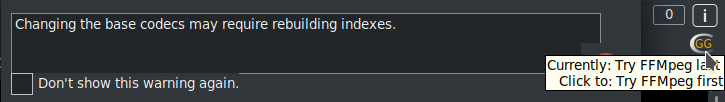
\includegraphics[width=0.7\linewidth]{images/ff_probe.png}
        \caption{Default warning when you click on FF icon in main window}
        \label{fig:ff_probe}
    \end{figure}
    \item[EDL version warns if mismatched] in the case of a Batch Render, it is often helpful to be warned if the EDL has been changed so that you are aware that what is going to be rendered is different than your current EDL session.
    \item[Create Bluray warns if not root] if checked and you are not logged in as root, you will get an error message in order to avoid doing a lot of work and then failing out because root is required for automount and to write on DVD hardware.
    \item[Popups activate on button up] this is the default but if unchecked, popups activate on button down.
    \item[Set Input Focus when window entered] this is checked on by default because on some operating system distros, when you move your mouse to a different window, nothing happens and you are left wondering why you can not enter information.  When checked this causes the input focus to shift to any Cinelerra window when the cursor enters an exposed region of the window which eliminates the need to switch input focus by tabbing. 
    \item[Click to activate text focus] Click to activate text focus
    \item [Click to deactivate text focus] if checked, you will have to click to deactivate text focus.
    \item[Always show next frame] in this mode the insertion pointer reflects the same as the Compositor so that for playing forward, the result is what looks like 1 was added to the frame displayed in the Compositor window.  This is fully explained in another section (\hyperref[sub:playing_seeking]{17.2.1}).
    \item[Use thumbnails in resource window] the Resource Window displays thumbnails of assets by default, but drawing asset thumbnails can take more time and CPU so you may want to uncheck this.
    \item[Perpetual session] is very useful for working on a project over many days so you can just quit before
    shutting down and the next time you start up Cinelerra you will be right back where you left off. You
    will retain all of your undo's and redo's.
    \item[Clears before toggle] when using copy/paste in drag and drop mode some users prefer to resort to the addition of the Ctrl key for adding multiple selections.  By checking this flag, the user retains usage as is commonly done for listbox operations.
    \item[Timeline Rectify Audio] for displaying rectified audio on the timeline instead of a standard audio waveform, check this flag.  The waveform is cut on the zero line, thus making the silent areas more visible and the waveform is stretched more over the entire height of the audio track, which improves the visibility of certain areas. This only affects the timeline and not any other audio waveform displays.
\end{description}

\section{About}%
\label{sec:about}

This section gives you information about the Cinelerra program and version you are running.  The original author’s copyright and name are first and foremost.  Next is a textbox with additional information and a summary of the monthly new features of note. Below that is a summary of the GPL License and the fact that it is provided without any warranty.  Then the licensing verbage is the item that you may need to refer to most often -- the \textit{built} date and time in case you need to know which version you are currently running.

\section{Environment Variables for Customization}%
\label{sec:environment_variables_customization}

Environment variables are global variables in the shell which all applications can read. They are set with a command like \texttt{set VARIABLE=value} or \texttt{export VARIABLE=value}. Environment variables can be viewed with a command like \texttt{env}.   The values set can be removed with \texttt{unset VARIABLE}.

The following exported variables can be set to customize your environment. \\ The \texttt{CIN\_CONFIG} variable could be extremely useful for testing purposes or for multiple users sharing the same home directory who would like different default preference settings.

\begin{description}
    \item[{\small CIN\_BROWSER}] name of browser to use by \textit{Shell Cmds} options
    \item[{\small CIN\_BROWSER}] configuration data; defaults to \texttt{\$HOME/.bcast5}
    \item[{\small CIN\_DAT}] location of data files, such as documentation, models, tip of the day
    \item[{\small CIN\_LADSPA}] LADSPA directory path; use colons to separate multiple paths; this is convenient to define an alternate directory if you share the same executable directory among computers via NFS.
    \item[{\small CIN\_LIB}] location of library programs, such as bdwrite
    \item[{\small CIN\_LOCALE}] locale text domain path to use for translating text
    \item[{\small CIN\_PLUGIN}] plugin directory path
    \item[{\small CIN\_RENDER}] complete filename with path, that was used for \textit{select file to render} to in the current session’s last successful Render job; this is used in the \texttt{RenderMux} defined \textit{Shell Cmds} and is available for any user-defined script inside Cinelerra
    \item[{\small CIN\_PKG}] used to set your text domain, that is the locale path pointing to mo language file
    \item[{\small CIN\_XSYNCH}] (for Developers only) set to 1 helps debugging for windows primitives to execute immediately and not be buffered up so you can see what is happening
\end{description}

One example:

\begin{lstlisting}[language=bash,numbers=none]
export CIN_BROWSER=chrome       #would override default firefox for Shell Cmds.
\end{lstlisting}

Another example:

\begin{lstlisting}[language=bash,numbers=none]
export CIN_CONFIG=/tmp/.bcast5   #use a temporary setup for testing purposes.
\end{lstlisting}

\begin{description}
    \item[{\small BC\_USE\_COMMERCIALS=1}] to activate the commercial database (db) methods.
    \item[{\small BC\_TRAP\_LV2\_SEGV}] to get a dump of the failure of an LV2 plugin for help in debugging.
    \item[{\small BC\_FONT\_SCALE=1.2}] for changing the default size of the characters to be twice as big.
    \item[{\small BC\_ICON\_SCALE=1.1}] for changing the default size of the icons to be bigger; can change \# to any. You can increase the size of the characters in the fonts and icons on your Cinelerra system.  This will make it easier to read the characters if you have trouble seeing the default small letters, which have been auto-scaled based on the window geometry. The user-friendly font/icon scaling default is 1 but you can set it to any decimal value.  To defeat default auto scaling and get any size characters/fonts, override the setting via the previous 2 listed shell environment variables. This is very sensitive, meaning that even a small increase in the numeric value can vary the size quite dramatically.
    \item[{\small BC\_FONT\_PATH=<colon-separated-search-path-for-fonts>}]  to add additional font sets for the \textit{Title}
    plugin or to remove all fonts set to : \texttt{(colon)}.  An example: \texttt{export BC\_FONT\_PATH=/usr/share/fonts}.
    \item[{\small BC\_FONT\_DEBUG=1}] debug for determining which font is causing problems.  0 for no debug.
    \item[{\small BC\_SCALE=1.2}] for setting up scaling for your monitor where you would like the text and icons to be bigger where 1.2 is a \# chosen accordingly; in this case the text and fonts will be 1.2 times the
normal size of 1. Refer to the previous Appearance section, \textit{Layout Scale} for more details.
    \item[{\small LADSPA\_PATH}] specify an alternate set of ladspa plugins or include the default with the use of a colon separated list of directories to search for LADSPA plugins. This is always used first and if it does not
    exist, then the value for \texttt{CIN\_LADSPA} becomes \texttt{LADSPA\_PATH}.
    \item[{\small LV2\_PATH}] specify a certain set of LV2 plugins to use.  Separate multiple paths with colons.
    \item[{\small LANG and LANGUAGE}] Cinelerra can be localized to display menus and messages in many languages. Language settings are normally read from your linux O/S language settings. To run on a language different than the one selected on your system just change the \texttt{LANG} and \texttt{LANGUAGE} environment variables.  For example, open a shell and type: \texttt{export LANG=es\_ES} or
    \texttt{LANGUAGE=es\_ES}, then run Cin from the same shell and you will have translations in Spanish.
    \item[{\small SHUTTLE\_CONFIG\_FILE}] alternate shuttle configuration file.
\end{description}

